\chapter{Implementation as a Browser Extension}
\label{sec.browserExtension}

As part of this thesis, a browser extension was developed that implements the detection methods presented in \autoref{sec.detection} and uses them to automatically analyze web pages that a user navigates to for any changes to \browserAPIs{}. As each of these approaches come with their own benefits and drawbacks, a combination of both of them will be used to improve the detection rate. The user is then informed about the result in the \ac{ui} through an icon that changes its color corresponding to the result (green, yellow, red). Additionally, clicking on this icon reveals a popup with a list of the affected APIs. While the extension can automatically detect \browserAPI{} manipulation and is simple to install and use, it is not able to classify whether the detected manipulation is legitimate or malicious, such as in the case of polyfills. This means that the extension is primarily aimed at web developers and security researchers that want to investigate the behavior of web applications and ensure that \browserAPIs{} are only overwritten when expected. The interpretation of a positive result – when manipulation was detected – unfortunately requires technical knowledge about the web application in question in order to know whether the manipulation is actually malicious or legitimate.

Even though in this case the detection tool was implemented in the form of a browser extension, the detection should ideally be builtin to the browser itself, as this would produce the most accurate results due to direct access to the internal memory state of the JavaScript context while also being isolated from it. However, not only is modifying and compiling a browser a considerably larger challenge than developing a browser extension, it also either requires the patch to be merged into the original (so-called “upstream”) code-base or constant maintenance to keep these patches compatible with the upstream. It is unlikely that such a patch would be merged into browsers and the alternative of patching and compiling a browser is not a viable solution to distribute the application for end users due to the required know-how and long compile times.

The first section \ref{sec.browserExtensionArchitecture} of this chapter will give an overview over the browser extension architecture and how its functionality was implemented. The second section \ref{sec.browserExtensionPolyfillDetection} will explain how the extension detects the use of polyfill libraries.

\filbreak{}

\section{Browser Extension Architecture}
\label{sec.browserExtensionArchitecture}

This section presents the architecture of the browser extension. An overview of the components and their interactions can be seen in \autoref{fig.browser-extension-context}.

\begin{figure}[H]
    \centering
    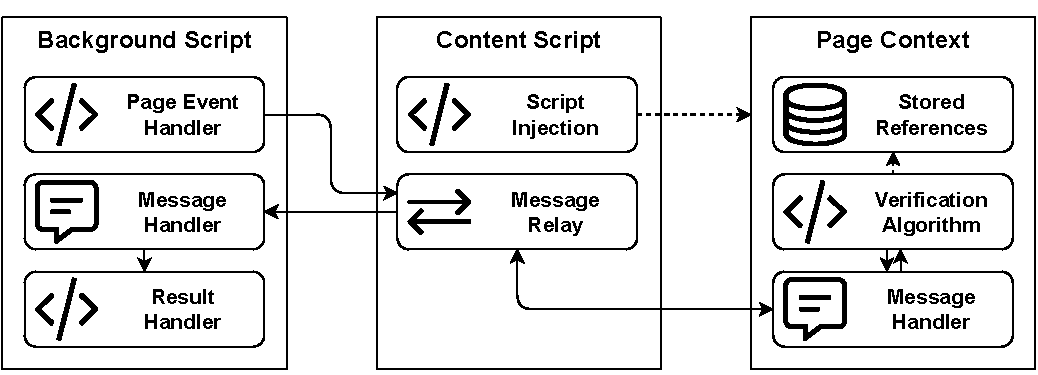
\includegraphics[width=16cm]{img/context-diagram.pdf}
    \caption{Browser extension architecture}
    \label{fig.browser-extension-context}
\end{figure}

The browser extension is responsible for injecting JavaScript code that makes use of the aforementioned detection mechanisms and displaying the results to the user. It is crucial that the code is injected and executed before any other code can be executed, including JavaScript code embedded in the original \acs{html} document itself.

Extensions are able to provide so-called “content scripts” which can access the \ac{dom}, but are sandboxed from the JavaScript context of the page and therefore also don't have access to the same \minline{window} object. In order to run code in the same context as the code of the page itself, a workaround is required: The content script creates a \minline{script} element and injects it into the \ac{dom} by prepending it to the \minline{head} or, as a fallback, the root \minline{document} element.
The desired code can either be provided by pointing the \minline{src} property to a script provided by the extension (which would need to be defined as a “web accessible resource“), or alternatively set the \minline{textContent} property to the string representation of the code. The latter allows dynamically creating the injected script, where one can make use of the fact that \minline{Function.prototype.toString()} returns the string representation of a function and \minline{JSON.stringify()} could be used to encode arguments passed to the function.

% \begin{lstlisting}[language=JavaScript,caption={Injecting JavaScript code into a page from a content script}]
% // Create new script element.
% const script = document.createElement("script");

% // Either provide a URL to the script
% script.src = browser.runtime.getURL("the-injected-script.js");
% // or provide the code as a string.
% const injectedFunction = () => {
%     // This will be executed in the page context.
%     window.foo = "bar";
% };
% const scriptAsString = "(" + injectedFunction.toString() + ")();";
% script.textContent = scriptAsString;

% // Prepend script to head, fallback to document root node.
% (document.head || document.documentElement).prepend(script);

% // Optionally, remove script after it was executed.
% script.remove();
% \end{lstlisting}

Another hurdle that gets in the way of script injection is the \hyperref[sec.csp]{\ac{csp} described in the fundamentals \autoref{sec.csp}}, which can be configured to deny execution of JavaScript code embedded into the \acs{html} document. While Chromium ignores the \ac{csp} for resources injected by extensions using the manifest v2 \acs{api}, this is no longer the case for extensions using manifest v3. Chromium manifest v3 extensions can instead directly execute code in the page context using \minline{chrome.scripting.executeScript()} with the \minline{ExecutionWorld} set to \minline{main}. However, this method can not be used here, since the provided code is no longer guaranteed to be executed first, which would allow JavaScript code to change properties before references are stored.

Firefox, unlike Chromium, treats resources injected by extensions the same way as page resources. This means that the extension only works when a page does not block inline scripts. A possible solution to this problem would be to use the Firefox-only Xray Vision \acs{api}, which allows direct access to a pages window object \cite{XrayVisionDocs}.

The next challenge is handling communication between the code running in the page context and the content script, in order for the extension to be able to request a verification and also get a result back. This can be solved by using \icode{window.postMessage()}, which allows posting a message that can contain any serializable Object to a given window. In both contexts a \icode{message} event listener is registered that checks received messages for a match and then acts accordingly.

Finally, the content script needs to relay messages between the page and the background script, which sends out the verification request after a page has finished loading and receives the response in order to display the results to the user. This communication happens in a similar manner, using the \icode{postMessage()} function of a \icode{runtime.Port} that connects both of the contexts.

The result is directly indicated to the user by the browser extension's action icon color. The icon is green when no changes to browser \acsp{api} are detected, yellow when there is no result, and red means that at least one change to a browser \acs{api} or other native function was detected.



\section{Polyfill Library Detection}
\label{sec.browserExtensionPolyfillDetection}

The browser extension detects polyfill libraries in two ways: scanning for the presence of global variable names that are used by polyfill libraries and by intercepting script inclusions if the \acs{url} matches patterns of known polyfill services.

It is possible to detect the polyfill library core-js due to a global variable that it creates. The library uses the global variable \icode{__core-js_shared__} to store information such as the version and certain function implementations in case different versions of the same library are used. As shown in \autoref{lst.detectcorejs}, the code for its detection only needs to check if the aforementioned variable name is a property of the global window object using the \icode{hasOwnProperty()} method.

\begin{lstlisting}[language=JavaScript,label={lst.detectcorejs},caption={Detection of the core-js library}]
if (Object.prototype.hasOwnProperty.call(window, "__core-js_shared__")) {
    // core-js detected
}
\end{lstlisting}

Some of the externally included polyfill libraries can be detected by filtering the scripts that a page includes and looking for \acsp{url} that match patterns of known polyfill services and library names. \autoref{lst.requestfilter} demonstrates how extensions can intercept requests using the \icode{webRequest.onCompleted} event. In order to limit events to scripts included by a page and requests originating fom JavaScript code, the type needs to be filtered to \icode{script} and \icode{xmlhttprequest}. The former type is assigned to requests for resources included using script elements, and the latter covers requests from scripts, which could in theory also be used to load and then execute JavaScript code. The listing also includes examples of patterns that are used to detect polyfill services, such as \icode{*://polyfill.io/*/} for the polyfill API \icode{polyfill.io}.

\filbreak{}

\begin{lstlisting}[language=JavaScript,label={lst.requestfilter},caption={Detecting external polyfill libraries through known \ac{url} patterns}]
browser.webRequest.onCompleted.addListener(details => {
    const origin = details.documentUrl || details.originUrl || details.initiator;

    console.log(origin, "made a request to", details.url);
}, {
    types: ["script", "xmlhttprequest"],
    urls: [
        // "polyfill" in path
        "*://*/*polyfill*",
        "*://*/*polyfill*?*",
        // polyfill APIs
        "*://polyfill.io/*/",
        "*://*.polyfill.io/*/",
        /* ... */
    ]
});
\end{lstlisting}
